

\section{Sensor de Pressão}
\label{pressao}


\begin{table}[ht!]

	\begin{tabular}{r l|l p{12cm} }
		
		\textcolor{gray}{Especificação} &&& 	{Sensor de Pressão - ??}\\
		\textcolor{gray}{Data} &&& 				{???}\\
        \textcolor{gray}{Beneficiado} &&&		{Velki} \\
        \textcolor{gray}{CNPJ} &&& 				{???} \\
        \textcolor{gray}{Número Nota} &&& 		{???} \\
		\textcolor{gray}{Quantidade} &&& 		{1} \\
		\textcolor{gray}{Valor} &&& 			{R\$1.6525,50} \\
		\textcolor{gray}{Data Sheet} &&& 		{-} \\

		\textcolor{gray}{Função no projeto} &&& {O sensor de pressão será utilizado para medir a profundidade do robô durante o processo de inserção da garra pescadora.} \\
		\textcolor{gray}{Razão da Escolha} &&& {   ?????   

		\begin{itemize}
		  \item \textbf{...} 
		  \item ...
		  \item ...
		\end{itemize}}
		

	\end{tabular}
\end{table}

%\begin{figure}[h!]
 %\centering
 %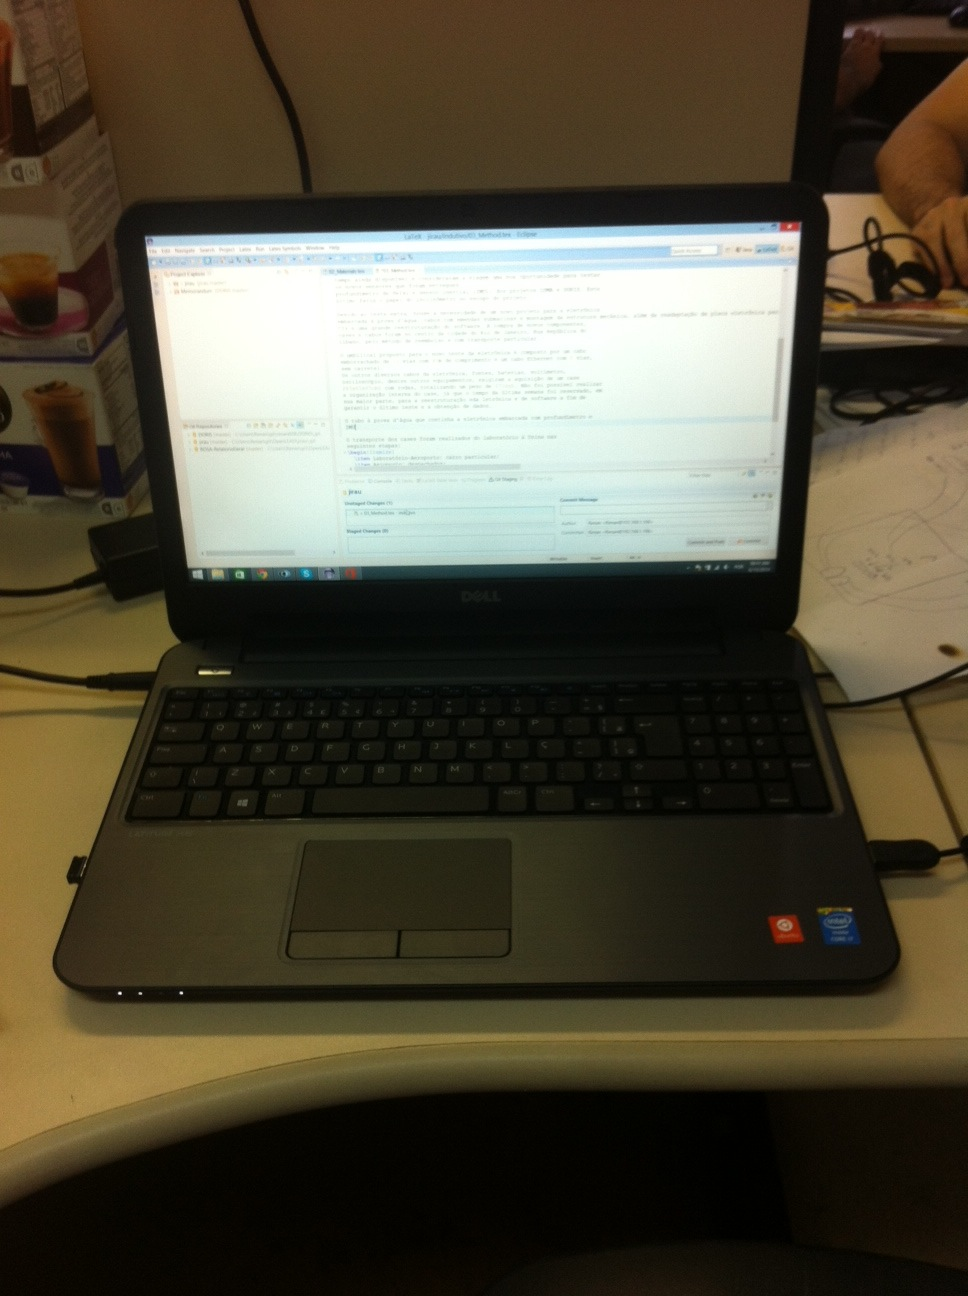
\includegraphics[width=0.5\columnwidth]{Notebook/foto.pdf}
 %\caption{Notebook Dell}  
%\end{figure}